
\chapter{Lager}

Zwischenlager der Texte die noch nicht aufgearbeitet wurden.

\subsection{gvim unterstützung einrichten}
\label{ssec:gvim-unterstuxfctzung-einrichten}

@todo: hier fehlt noch die beschreibung@

\begin{itemize}
\itemsep1pt\parskip0pt\parsep0pt
\item
  erstellen der startdatei
\item
  einrichten
\end{itemize}


% dieser teil wurde ausgeblendet da bei der übernahme
% von pandoc noch fehler auftreten

%\subsubsection{autosave funktion}\label{autosave-funktion}
%
%mit dem plugin autosave kann man rumex auch dazu bringen dateien nicht
%nur automatisch zu speichern sondern auch gleich die html datei zu
%erstellen.
%
%jedoch ist eine kleine änderung am plugin notwendig.
%
%\begin{shaded}
%\begin{highlighting}[]
%\keywordtok{diff --git a/plugin/autosave.vim b/plugin/autosave.vim}
%\normaltok{index f09a904..ec2f463 100644}
%\datatypetok{--- a/plugin/autosave.vim}
%\datatypetok{+++ b/plugin/autosave.vim}
%\datatypetok{@@ -11,6 +11,12 @@ else}
%   \normaltok{let g:auto_save_loaded = 1}
% \normaltok{endif}
% 
%\othertok{+if exists("g:rumex")}
%\othertok{+  finish}
%\othertok{+else}
%\othertok{+  let g:rumex = 0}
%\othertok{+endif}
%\othertok{+}
% \normaltok{let s:save_cpo = &cpo}
% \normaltok{set cpo&vim}
% 
%\datatypetok{@@ -33,10 +39,14 @@ function! autosave()}
%   \normaltok{if g:auto_save >= 1}
%     \normaltok{let was_modified = &modified}
%     \normaltok{silent! wa}
%\stringtok{-    if was_modified && !&modified}
%\stringtok{-      echo "(autosaved at " . strftime("%t") . ")"}
%\stringtok{-    endif}
%\stringtok{-  endif}
%\othertok{+   if was_modified && !&modified}
%\othertok{+       if g:rumex == 1}
%\othertok{+           silent! make html}
%\othertok{+           echo "html datei wurde erstellt"}
%\othertok{+       endif}
%\othertok{+       echo "(autosaved at " . strftime("%t") . ")"}
%\othertok{+   endif}
%\othertok{+endif}
% \normaltok{endfunction}
% 
% \normaltok{function! autosavetoggle()}
%\end{highlighting}
%\end{shaded}
%
%mit dem befehl \texttt{:let rumex=1} bzw. \texttt{let rumex=0} kann das
%erstellen der html datei ein bzw. ausgeschaltet werden.
%
%installiert man sich dann noch im firefox dann noch die erweiterung.
%``tab auto reload'' werden die änderungen im browser immer gleich
%angezeigt.
%
%über die nutzbarkeit kann man sich streiten da nach einem html lauf der
%cursor immer an den anfang der zeile, in der man sich gerade befindet,
%springt. mir ist die variante mit \texttt{\textless{}f5\textgreater{}}
%lieber. die ``tab auto reload'' funktion im firefox verwende ich aber
%schon sehr gerne.

\subsubsection{tipps zur benutzung gvim}\label{tipps-zur-benutzung-gvim}

\subsubsection{vim kurztasten}\label{vim-kurztasten}

eine übersicht der rumex kurztasten für den editor vim findest du auf
der seite \href{vim-kurztasten.htm}{vim-kurztasten}.

\subsubsection{gvim menü}\label{gvim-menuxfc}

eine übersicht des rumex menüs für den editor gvim findest du auf der
seite \href{gvim-menue.htm}{gvim-menü}.

\paragraph{dateiname ergänzen}\label{dateiname-erguxe4nzen}

will man in die datei einen dateinamen einbauen, weiß aber nicht mehr
genau wie er heißt, kann man folgenden trick verwenden. in diesem
beispiel wird ein bildname gesucht. im text schreibe man
\texttt{../bilder/tw} und drückt dann die tastenkombination
\texttt{c-x + c-f}, gvim öffnet ein dialogfeld in dem alle dateien die
auf dieses muster übereinstimmen geöffnet. gibt es nur einen treffer
wird dieser gleich eingefügt.

\paragraph{wort innerhalb des dokumentes
suchen}\label{wort-innerhalb-des-dokumentes-suchen}

sucht man ein wort das man im dokument schon einmal verwendet hat, um
zum beispiel darauf zu verweisen. schreibt man den wortanfang und drückt
dann \texttt{c-p}. es öffnet sich ein dialogfeld in dem alle wörter die
auf dieses muster passen angezeigt werden. gibt es nur einen treffer
wird dieser gleich eingefügt.

\paragraph{nützliche erweiterungen}\label{nuxfctzliche-erweiterungen}

vim bietet ein paar nützliche erweiterungen in form von plugins an. hier
eine liste, der plugins, die ich gerne verwende.

\begin{description}
\item[pathogen.vim]
diese erweiterung macht das installieren weitere erweiterungen einfach.
dabei ist die installation von \texttt{pathogen} schnell erledigt.

%\begin{shaded}
%\begin{highlighting}[]
%\keywordtok{mkdir} \normaltok{-p ~/.vim/autoload ~/.vim/bundle }
%\keywordtok{wget} \normaltok{-o ~/.vim/autoload/pathogen.vim //}
%\keywordtok{http}\normaltok{://www.vim.org/scripts/download_script.php?src_id=16224}
%\end{highlighting}
%\end{shaded}

in die \texttt{.vimrc} muss dann noch nachfolgende zeile eingebaut
werden.

\begin{verbatim}
call pathogen#infect()
\end{verbatim}

eingebaut werden.

jetzt braucht man die erweiterungen nur mehr in das verzeichnis
\texttt{.vim/bundle} zu kopieren und vim neu starten. in verbindung mit
\texttt{git} wieder eine einfache sache.

%\begin{shaded}
%\begin{highlighting}[]
%\keywordtok{cd} \normaltok{~/.vim/bundle}
%\keywordtok{git} \normaltok{clone https://github.com/vim-pandoc/vim-pandoc.git}
%\end{highlighting}
%\end{shaded}

\item[vim-pandoc]
erweiterung rund um pandoc.
\item[fuzzyfinder]
dateien schnell zum editieren öffnen. installiert ist diese erweiterung,
vorausgesetzt man verwendet pathogen, mit dem befehl:

\begin{verbatim}
wget -o /tmp/vim-fuzzyfinder.zip http://www.vim.org/scripts/download_script.php?src_id=10588
mkdir ~/.vim/bundle/vim-fuzzyfinder
unzip /tmp/vim-fuzzyfinder.zip -d ~/.vim/bundle/vim-fuzzyfinder/
\end{verbatim}

für das öffnen dies datei dialogs sollte man sich dann noch eine
kurztaste konfigurieren.

\begin{verbatim}
" -------------------------------------------------------------
" fuzzyfinder file suche auf <f12> binden
map <f12> :fuzzyfinderfile <cr>
\end{verbatim}
\end{description}

\subsection{seite auf einem github.com server
einrichten}\label{seite-auf-einem-github.com-server-einrichten}

@todo

\begin{itemize}
\itemsep1pt\parskip0pt\parsep0pt
\item
  einrichten eines github.com zugangs
\item
  arbeits- repository auf den ap\footnote{mit ap ist der
    \textbf{a}rbeits\textbf{p}latz rechner gemeint.} holen
\item
  die rumex zip datei
\item
  die dateien des zip archives in das arbeits- repository kopieren
\item
  grund dateien anpassen

  \begin{itemize}
  \itemsep1pt\parskip0pt\parsep0pt
  \item
    @fixme: angabe welche dateien fehlt noch@
  \end{itemize}
\item
  erste änderungen vornehme
\item
  \texttt{make online} - fertig.
\end{itemize}

\subsection{seite auf einem nicht github.com server
einrichten}\label{seite-auf-einem-nicht-github.com-server-einrichten}

\subsubsection{datei upload per git}\label{datei-upload-per-git}

@todo

auf der seite \href{http://rumex.it-bayer.de}{rumex.it-bayer.de} findet
man eine beschreibung wie man den rumex baukasten auf einen
\textbf{nicht} \texttt{github.com} server installiert.

\subsubsection{datei upload per ftp}\label{datei-upload-per-ftp}

@todo

\section{aufbau des rumex baukastens}\label{aufbau-des-rumex-baukastens}

@todo

\subsection{root verzeichnis}\label{root-verzeichnis}

im \texttt{root} verzeichnis findet man alle \texttt{html} dateien der
seite. diese werde vom baukasten erstellt und müssen nicht von hand
verändert werden. zusätzlich findet man noch ein folgende systemdateien:

\begin{description}
\item[rss.xml]
news feed datei, wird vom system erstelle
\item[readme.md]
beschreibungsdatei die von github.com gebraucht wird
\item[robots.txt]
datei für die suchmaschinen
\item[favicon.ico]
icon für den browser
\item[.htaccess]
konfiguration für den apache server
\item[cname]
@fixme: beschreibung@
\end{description}

\subsection{unterverzeichnisse}\label{unterverzeichnisse}

\begin{description}
\item[.rumex/]
@fixme: beschreibung@
\item[.rx/]
@fixme: beschreibung@
\item[rxtpl/]
standard template verzeichnis. in diesem verzeichnis befinden sich die
dateien die für das aussehen der seite verantwortlich sind.

folgende dateinen und verzeichnisse sind hier zu finden

\begin{itemize}
\itemsep1pt\parskip0pt\parsep0pt
\item
  index.html (weiterleitung zum root verzeichnis)
\item
  css/\\
\item
  js/
\item
  img/
\end{itemize}
\item[bilder/]
in diesem verzeichnis werden alle bilder der seite abgelegt.
\end{description}

\subsection{steuerung durch
dateiendung}\label{steuerung-durch-dateiendung}

das aussehen der dateien bezüglich des inhaltsverzeichnisses könnte auch
durch die dateiendung gesteuert werden.

\subsubsection{beispiel}\label{beispiel}

\begin{description}
\item[datei.rx0s]
würde eine html datei ohne inhaltsverzeichnis erstellen.
\item[datei.rx1s]
erstellt die html datei mit dem inhaltsverzeichnis aus den einträgen der
h1 überschriften.
\item[datei.rx2s]
erstellt eine html datei mit dem inhaltsverzeichnis aud den einträgen
der h1 und h2 überschriften.
\end{description}

zusätzlich könnte die dateiendung auch eine unterschiedliche verwendung
der dateien ermöglichen.

\begin{description}
\item[datei.rx0s, datei.rx1s \ldots{}]
standard datei.
\item[datei.rx0x, datei.rx1x \ldots{}]
datei die nicht in die liste auf \texttt{index.html} eingebunden wird.
\item[datei.rx0v, datie.rx1v \ldots{}]
versteckte datei. diese taucht weder in der \texttt{index.html} noch in
der \texttt{sitemap.xml} auf.
\item[datei.rx0w]
datei mit einer weiterleitung. die weiterleitung wird dabei mittels
\texttt{javascript} realisiert, da github keine \texttt{.htaccess}
weiterleitung unterstützt.

\begin{verbatim}
% weiterleitung nach beschreibung.html
%
%

<script language="javascript">
<!--
window.location.href="beschreibung.html";
// -->
</script> 
\end{verbatim}
\end{description}

bei der änderung der dateiendung bleibt der eigentliche \texttt{html}
name gleich. nur die funktion der einbindung ändert sich.

\subsection{sonderseiten}\label{sonderseiten}

im verzeichnis \texttt{pandoc} befinden sich sonderseiten.

\begin{description}
\item[rumex/index.rx0x]
diese datei wird vom programm \texttt{.bin/make\_index.pl} erstellt,
muss somit nicht vorhanden sein.
\item[rumex/start.rx0s]
die \texttt{start.rx0s} wird als vortext in die \texttt{index.rx0x}
eingebunden. mit ihr kann man oberhalb der seiten liste einen extra text
in die \texttt{index.html} eingebunden werden.\\\textbf{diese datei ist
erforderlich und muss vorhanden sein.}
\item[rumex/rss.rx0x]
datei für die rss feed funktion.
\item[rumex/impressum.rx0x]
datei für die impressumsangaben.\\\textbf{ist nicht zwingend
erforderlich. jedoch muss die \texttt{.inc/fuss.html} entsprechende
bearbeitet, der link muss raus genommen, werden.}
\item[rumex/makefile]
sie \texttt{make} steuerdatei.
\end{description}

\subsection{aufbau der startseite}\label{aufbau-der-startseite}

die startseite \texttt{markdown/start.rx0s} muss vorhanden sein. es
reicht auch ein `touch markdown/start.rx0s.

der normale aufbau könnte so ausschauen. die \texttt{pandoc} kopfzeile
sind nicht zwingend erforderlich.

\begin{verbatim}
% start.rx0s
%
%

hier kommt auch schon der vortext für die index.html
\end{verbatim}

\subsection{aufbau der einzelseiten}\label{aufbau-der-einzelseiten}

die einzelseiten liegen alle im verzeichnis \texttt{rumex} und zwar in
der sprache \texttt{markdown} bzw. der erweiterung von \texttt{pandoc}.

diese einzelseiten werden in chronologischer reihenfolge in die
startseite \texttt{index.html} eingebunden und bilden sozusagen das
inhaltsverzeichnis der seite. in jeder einzelseite wird dazu ein
sogenannter \emph{``vortext''} hinterlegt. die seite bzw. der kopf der
seite hat dabei folgenden aufbau.

\begin{verbatim}
% seiten überschrift 1
% seiten überschrift 2
% seiten überschrift 3

<!--


# listen-überschrift

überschrift und text der in der listenübersicht
auf index.html angezeigt wird.

alles was innerhalb der html kommentar marken
steht wird nur auf der index.html seite angezeigt.

-->

alles was sich außerhalb der html marken
befindet wird auch auf der eigentlichen seite angezeigt.

durch das schlüsselwort "schnipp", das auch in html
kommentar marken stehen muss, wird der vortext beendet.
auf der index.html erscheint an dieser stelle der link
"... weiter lesen".

<!-- schnipp -->

ab hier geht dann der inhlat der eigentlichen seite los.
\end{verbatim}

\subsection{template}\label{template}

@todo

änderung gegenüber des original \texttt{pandoc} templates.

%\begin{shaded}
%\begin{highlighting}[]
%\datatypetok{5c5,8}
%\stringtok{<   <meta name="generator" content="pandoc">}
%\keywordtok{---}
%\othertok{>   <!-- rumex version -->}
%\othertok{>   <meta name="generator" content="$meta_generator$">}
%\othertok{>   <!-- rumex suchmaschine -->}
%\othertok{>   <meta name="robots" content="$meta_robots$">}
%\datatypetok{30a34,35}
%\othertok{>   <!-- rumex rss -->}
%\othertok{>   <link rel="alternate" type="application/rss+xml" title="$rsstitel$" href="$rssfile$" />}
%\datatypetok{41c46}
%\stringtok{< <h1 class="title">$title$</h1>}
%\keywordtok{---}
%\othertok{> <h1 class="title"><a title="zur startseite" href="index.html">$title$</a></h1>}
%\datatypetok{43c48}
%\stringtok{< <h2 class="author">$author$</h2>}
%\keywordtok{---}
%\othertok{> <h2 class="author"><a title="zur startseite" href="index.html">$author$</a></h2>}
%\datatypetok{46c51}
%\stringtok{< <h3 class="date">$date$</h3>}
%\keywordtok{---}
%\othertok{> <h3 class="date"><a title="zur startseite" href="index.html">$date$</a></h3>}
%\datatypetok{54a60}
%\othertok{> <div id=seite>}
%\datatypetok{55a62}
%\othertok{> </div>}
%\end{highlighting}
%\end{shaded}

\section{rss feed funktion}\label{rss-feed-funktion}

@todo

wird nicht aus den einzelnen dateien erstellt sondern muss manuell
editiert werden, datei \texttt{.rx/rss.rx0x}.

jede überschrift eines eintrags muss mit einem \texttt{\{.nn1\}} enden.

danach kommen die angaben zu:

\textbf{link:} \emph{verweis zur seite mit weiteren
informationen}\\\textbf{autor:} \emph{autor der den eintrag geschrieben
hat}\\\textbf{kategorie:} \emph{kategoie des eintrags}\\\textbf{datum:}
\emph{datum des eintrags.} das richtige format bekommt man mit dem
befehl \texttt{date -r}.

die in html kommentar marker eingeschlossen sind.

anschließend folgt die meldung. zur zeit werden folgende \texttt{pandoc}
formatierungen unterstützt.

\begin{itemize}
\itemsep1pt\parskip0pt\parsep0pt
\item
  überschriften ab der stufe 3 \texttt{\#\#\#}
\item
  aufzählungen \texttt{-}
\item
  aufzählungen \texttt{*}
\item
  zitate \texttt{\textgreater{}}
\item
  links \texttt{{[}link{]}(http://muster.tdl)}. diese dürfen nicht am
  anfang einer zeile stehen.
\item
  bilder \texttt{!{[}bild{]}(../bilder/muster.png "muster.png")}, diese
  dürfen nicht am anfang einer zeile stehen.
\item
  code `code`.
\end{itemize}

\subsection{beispiel einer rss feed
seite}\label{beispiel-einer-rss-feed-seite}

%\begin{shaded}
%\begin{highlighting}[numbers=left,,firstnumber=100,]
% \normaltok{% abo seite - newsletter - rss feed}
% \normaltok{% }
% \normaltok{%}
% 
% \normaltok{<!--}
% \normaltok{| titel: rumex - ein home page baukasten}
% \normaltok{| beschreibung: aktuelles und neuigkeiten vom rumex home page baukasten}
% \normaltok{| klink: http:}\commenttok{//www.it-bayer.de/rumex/}
% \normaltok{| lang: de-de}
% \normaltok{| bildtitel: it-bayer rumex meldungen}
% \normaltok{| bildurl: http:}\commenttok{//www.itbayer.de/rumex/bilder/404.png}
% \normaltok{| bildlink: http:}\commenttok{//www.it-bayer.de/rumex/}
% \normaltok{| bildbeschreibung: aktuelles und neuigkeiten von der rumex seite.}
% \normaltok{-->}
% 
% \errortok{# rumex bekommt die rss feed funktion\{.rssfeed1\}}
% 
% \normaltok{<!-- }
% \normaltok{| link: http:}\commenttok{//www.it-bayer.de/rumex/}
% \normaltok{| autor: it-bayer}
% \normaltok{| kategorie: neues}
% \normaltok{| datum: thu, }\decvaltok{04} \normaltok{jul }\decvaltok{2013} \decvaltok{10}\normaltok{:}\decvaltok{07}\normaltok{:}\decvaltok{06} \normaltok{+}\decvaltok{0200}
% \normaltok{-->}
% 
% \normaltok{in den rumex baukasten wurde eine rss feed funktion eingebaut.}
% \normaltok{die einträge werden dabei auch aus einem `pandoc` dokument gelesen}
% \normaltok{und nach `rss.xml` geschrieben.}
% 
% \normaltok{zusätzlich ist diese datei auch als `rss.html` unter }
% \normaltok{<http:}\commenttok{//www.it-bayer.de/rumex/rss.html> verfügbar.}
%\end{highlighting}
%\end{shaded}

\subsection{rss dateiname}\label{rss-dateiname}

der dateiname ist mit \texttt{rss.xml} vorbelegt und kann über die
variable \texttt{rss\_file} in der \texttt{config.md} geändert werden.

\subsection{rss titel}\label{rss-titel}

der title des rss feed wird durch die variable \texttt{rss\_titel}
angepasst.

\begin{verbatim}
rss_titel = "neuigkeiten von rumex baukasten"
\end{verbatim}

\subsection{rss auslagern}\label{rss-auslagern}

den rss link kann man auch auslagern so dass dieser auf eine andere
seite zeigt. dazu setzt man die variable \texttt{rss\_extern} mit dem
entsprechenden link. die variabel \texttt{rss\_file} wird dadurch nicht
mehr verwendet. auch der rss lauf wird dadurch ausgeschaltet und durch
eine meldung ersetzt.

\subsection{rss kurztaste}\label{rss-kurztaste}

für die einzelnen einträge steht auch eine kurztaste \texttt{.rnn} zur
verfügung.\\in gvim unter

\begin{verbatim}
rumex -> textbausteine -> neuernews eintrag
\end{verbatim}

eingefügt wird dann folgende vorgabe. der wert hinter datum wird von
system ausgelesen und entsprechende gesetzt.

\begin{verbatim}
 # neue nachricht{.nn1}

<!--
| link: http://www.it-bayer.de/rumex/
| autor: it-bayer
| kategorie: neues
| datum: mon, 28 oct 2013 07:36:56 +0100
-->

ab hier geht die neue nachricht los.
\end{verbatim}

\subsection{interna}\label{interna}

durch die beschriebenen rss variablen wird die erstellung des rss feed
gesteuert. es wird in jede html datei nachfolgender header abschnitt
eingebaut wenn die \texttt{rss\_title} variable gesetzt wurde.
\texttt{rss\_file} bzw. \texttt{rss\_extern} steuern den \texttt{href}
eintrag.

%\begin{shaded}
%\begin{highlighting}[]
%\commenttok{<!-- rumex rss -->}
%\keywordtok{<link}\othertok{ rel=}\stringtok{"alternate"}\othertok{ type=}\stringtok{"application/rss+xml"}\othertok{ title=}\stringtok{"neuigkeiten von rumex baukasten"}\othertok{ href=}\stringtok{"rss.xml"} \keywordtok{/>}
%\end{highlighting}
%\end{shaded}

\section{rumex auf einem usb stick}\label{rumex-auf-einem-usb-stick}

rumex kann auch auf einem usb stich installiert werden. der stick muss
aber ein dateiformat besitzt\\welches mit dateirechten und symbolische
links umgehen kann.

\textbf{usb sticks im vfat format funktionieren nicht.} man kann zwar
die daten darauf ablegen. das arbeiten über den stick funktioniert nicht
wirklich. auch wenn man die daten, von einem vfat stick, auf ein *nix
system kopiert werden muss händisch nach gebessert werden.

linktipp:
\href{http://www.it-bayer.de/usb-stick.html?suchwort=versch\#usb-stick-unter-linux-verschl\%c3\%bcsseln}{usb
stick unter linux verschlüsseln}

\section{make steuerung}\label{make-steuerung}

@todo

gesteuert wird der baukasten mittels \texttt{make} im unterverzeichnis
\texttt{rumex}. folgende \texttt{make} befehle stehen dabei zur
verfügung.

\begin{description}
\item[make html]
erstellt die einzelnen html dateien. hier kann auch nur \texttt{make}
verwendet werden.
\item[make index]
erstellt die \texttt{index.md} datei aus der dann die
\texttt{index.html} datei erstellt wird.
\item[make all]
eine zusammenstellung aus \texttt{make index} und \texttt{make html}.
\item[make online]
daten auf github hoch laden.
\item[make bilder]
erstellt bilder in verschiedenen auflösungen.
\end{description}

\section{update}\label{update}

@todo

\section{homepage änderung, schnell und immer
aktuell}\label{homepage-uxe4nderung-schnell-und-immer-aktuell}

wer wünscht es sich nicht einen schnellen zugriff auf seine homepage.
sei es um schnell was zu ändern oder genauso schnell was neues
einzustellen. rumex bietet in verbindung mit \texttt{tilda} eine schöne,
einfache und auch schnelle lösung.

\begin{figure}[htbp]
\centering
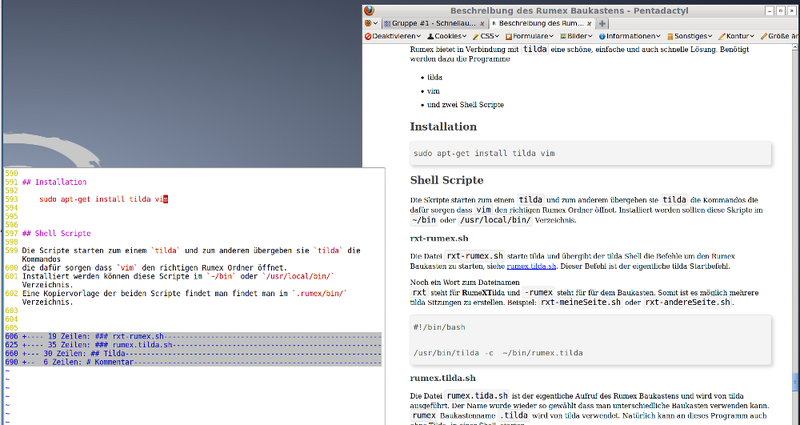
\includegraphics{../bilder/rumex-tilda_800_.png}
\caption{rumex im tilda fenster. mit einem tastendruck öffnet sch das
tilda fenster und man kann die texte eintippen. ein erneuter tastendruck
schließt das tilda fenster wieder und der bildschirm ist wieder frei.
hat man seine änderung abgeschossen kann man mit den rumex
\href{vim-kurztasten.html}{vim kurztasten} die änderung schnell online
stellen.}
\end{figure}

\subsection{installation der tilda
unterstützung}\label{installation-der-tilda-unterstuxfctzung}

die installation ist nicht umfangreich. man braucht vim und tilda und
dann noch zwei bash script. eine kopiervorlage der beiden scripte findet
man findet man im \texttt{.rumex/bin/} verzeichnis.

\begin{verbatim}
sudo apt-get install tilda vim
cp .../rumex/.rumex/bin/rxt-rumex.sh ~/bin/.
cp .../rumex/.rumex/bin/rumex-tilda.sh ~/bin/.
\end{verbatim}

diese beiden bash scripte müssen anschließend noch angepasst werden.

\subsubsection{shell scripte}\label{shell-scripte}

die scripte starten zum einem \texttt{tilda} und zum anderem übergeben
sie \texttt{tilda} die kommandos die dafür sorgen \texttt{vim} im
richtigen rumex ordner zu öffnet. installiert werden können diese
scripte im \texttt{\textasciitilde{}/bin} oder \texttt{/usr/local/bin/}
verzeichnis.

\paragraph{rumex-tilda.sh}\label{rumex-tilda.sh}

die datei \texttt{rumex-tilda.sh} starte tilda und übergibt der tilda
shell die befehle um den rumex baukasten zu starten, siehe
\hyperref[rumex.vim.sh]{rumex.vim.sh}.

\begin{verbatim}
#!/bin/bash

/usr/bin/tilda -c  ~/bin/rumex-vim.sh
\end{verbatim}

\paragraph{rumex-vim.sh}\label{rumex-vim.sh}

mit dem befehl \texttt{rumex-vim.sh} wird der rumex baukastens
aufgerufen. dieser befehl wird unter anderem auch von
\texttt{rumex-tilda.sh} verwendet. \texttt{rumex-vim.sh} kann natürlich
auch in einem shellfenster ausgeführt werden.

\paragraph{rumex-gvim.sh}\label{rumex-gvim.sh}

mit dem befehl \texttt{rumex-gvim.sh} wird der rumex baukasten mit dem
editor gvim gestartet.

\subsection{tilda einrichten}\label{tilda-einrichten}

nach dem ersten start wird tilda in linken oberen bildschirm bereich
eingeblendet. man sollte tilda nun noch an seine bedürfnissen anpassen.
dazu in das tilda fenster mit der rechten maustaste klicken und
\texttt{eigenschaften} aus wählen.

\textbf{übrigens:} man kann \texttt{tilda} mehrfach starten. somit kann
auf mehreren rumex installationen parallel über diese weiße zugegriffen
werden. man sollte nur jede \texttt{tilda} sitzung ein wenig anders
konfigurieren.

\textbf{nachteil:} ein nachteil von \texttt{tilda} darf man aber nicht
verschweigen. bei wechseln zwischen den fenstern kann man die
tastenkombination
\texttt{\textless{}alt\textgreater{}+\textless{}tab\textgreater{}} nicht
verwenden bzw. man kommt mit dieser kombination nicht mehr zurück nach
\texttt{tilda}. schließt und öffnet man \texttt{tilda} mit der
definierten taste bekommt man aber den fokus wieder in das fenster.

will man die
\texttt{\textless{}alt\textgreater{}+\textless{}tab\textgreater{}}
kombination doch verwenden muss man die standardeinstellung von tilda
ändern. den erforderlichen schalter findet man in der konfiguration,
reiter \emph{allgemein} -\textgreater{} schalter \emph{nicht in der
taskleiste anzeigen}.



\section{Warum wurde diese Beschreibung nicht mit Rumex erstellt}

Eigentlich sollte Rumex sich auch selber beschreiben.
Bei der Erstellung meiner \emph{Sensen Denkschrift} ist mir Rumex 
jedoch zu klein geworden. 
Große Dokumente sind mit Rumex nicht mehr so einfach zu handeln.
Da es sich bei der Rumex Beschreibung auch um ein großes Dokument handelt. Es wächst zumindest immer weiter. Bin ich auf meine Vorlage für tex4ht umgestiegen.
Ich kann somit die Texte mit einem Programm wie
Texstudio%
\footnote{Obwohl mir beim Texstudio deii Tasten zur Navigation,
wie ich sie von vim gewohnt bin, fehlen.} 
bearbeiten und fühle mich bei der Bearbeitung 
größere Dokumente einfach wohler.

Außerdem finde ich die PDF Ausgabe mittels KOMA-Scripts auch 
schöner als die von Pandoc.


